% ============================================================
% Corrigé du TP : La loi normale au service du contrôle de fabrication -- butée
% Pôle Formation UIMM - CVDL - BTS CPRP - S. JAUBERT
% Énoncé : MOD08_TP_CPRP_Capabilite_Butee_v1_0
% ============================================================
\documentclass[a4paper,11pt]{article}
% Préambule commun TP / corrigé -- MOD08 TP CPRP capabilité d'une butée
\usepackage[utf8]{inputenc}
\usepackage[T1]{fontenc}
% babel-french absent sur certains postes : chargement conditionnel
\IfFileExists{french.ldf}{\usepackage[french]{babel}}{}
\usepackage{helvet}
\usepackage{courier}
\renewcommand{\familydefault}{\sfdefault}
\usepackage[top=3cm, bottom=2.5cm, left=2cm, right=2cm, headheight=2cm]{geometry}
\usepackage{amsmath,amssymb,amsfonts}
\usepackage{graphicx}
\usepackage[dvipsnames,table]{xcolor}
\usepackage{tikz}
\usepackage{pgfplots}
\pgfplotsset{compat=1.16}
\usepackage[most]{tcolorbox}
\usepackage{fancyhdr}
\usepackage{enumitem}
\usepackage{array,needspace,booktabs}
\usepackage{titlesec}
\usepackage{hyperref}

\definecolor{uimmblue}{HTML}{005C85}
\definecolor{uimmred}{HTML}{D31326}
\definecolor{uimmlightblue}{HTML}{E8F1F8}
\definecolor{uimmgray}{HTML}{333333}
\definecolor{uimmlightgray}{HTML}{F5F5F5}
\definecolor{ctlgreen}{HTML}{2E8B3D}
\hypersetup{colorlinks=true, linkcolor=uimmblue, urlcolor=uimmblue}

\titleformat{\section}{\Large\bfseries\color{uimmblue}}{}{0pt}{}[\vspace{2pt}{\color{uimmblue}\titlerule[1.2pt]}]
\titleformat{\subsection}{\large\bfseries\color{uimmblue}}{}{0pt}{}
\setlist[enumerate,1]{label={\color{uimmblue}\textbf{\arabic*.}}, leftmargin=*}
\setlist[enumerate,2]{label=\alph*), leftmargin=*}
\setlist[itemize,1]{label={\color{uimmblue}\textbullet}}

\newtcolorbox{exo}[1]{colback=white, colframe=uimmblue, fonttitle=\bfseries\color{white},
  coltitle=white, title={#1}, boxrule=1pt, arc=2pt,
  left=8pt, right=8pt, top=5pt, bottom=6pt, before skip=10pt, after skip=6pt}
\newtcolorbox{consigne}{colback=uimmlightgray, colframe=uimmgray, boxrule=0.8pt, arc=3pt,
  left=8pt, right=8pt, top=6pt, bottom=6pt}
\newtcolorbox{rappel}[1]{colback=uimmlightblue, colframe=uimmblue, fonttitle=\bfseries\color{white},
  coltitle=white, title={#1}, boxrule=0.8pt, arc=2pt,
  left=8pt, right=8pt, top=4pt, bottom=4pt, before skip=7pt, after skip=6pt}

\newcommand{\calc}{\,{\color{uimmred}\small\textbf{[calculatrice]}}}
\newcommand{\tabl}{\,{\color{uimmred}\small\textbf{[tableur ou R]}}}
\newcommand{\duree}[1]{\hfill{\normalsize\color{uimmred}#1}}
\newcommand{\Dbar}{\overline{D}}
\newcommand{\Dbb}{\overline{\overline{D}}}
\newcommand{\Rbar}{\overline{R}}
% Zone de réponse lignée : #1 = nombre de lignes
\newcommand{\zone}[1]{\par\smallskip\noindent\begin{tikzpicture}
  \foreach \i in {1,...,#1}{\draw[uimmgray!30] (0,-0.74*\i) -- (\linewidth-1pt,-0.74*\i);}
  \end{tikzpicture}\par\smallskip}
\newcommand{\EnTete}[1]{%
\pagestyle{fancy}\fancyhf{}\renewcommand{\headrulewidth}{0pt}
\fancyhead[L]{\raisebox{-0.5\height}{
\includegraphics[height=1.5cm]{logo_uimm_placeholder.jpg}}}
\fancyhead[C]{\begin{minipage}{8cm}\centering
  {\small\color{uimmblue}\textbf{Pôle Formation UIMM - CVDL}}\\
  {\footnotesize\color{uimmgray} BTS CPRP -- Mathématiques}\end{minipage}}
\fancyhead[R]{{\small\color{uimmblue}\textbf{MOD08 -- #1}}}
\fancyfoot[C]{{\color{uimmblue}\rule{\textwidth}{1pt}}\\[2pt]
  {\footnotesize\color{uimmgray} Pôle Formation UIMM -- Centre-Val de Loire \hfill S. JAUBERT \hfill \thepage}}}
% Cartes de contrôle vierges (dossier réponse) : #1 = légende y, ymin, ymax, pas
\pgfplotsset{ctl/.style={width=0.93\linewidth, height=6.3cm, xmin=0.5, xmax=6.5, xtick={1,2,3,4,5,6},
  grid=both, minor y tick num=4, grid style={uimmgray!35}, minor grid style={uimmgray!15},
  xlabel={Numéro de l'échantillon}, tick label style={font=\footnotesize},
  /pgf/number format/use comma, /pgf/number format/fixed, /pgf/number format/precision=3,
  /pgf/number format/fixed zerofill, scaled y ticks=false,
  xticklabel={\pgfmathprintnumber[fixed,precision=0]{\tick}}}}
\EnTete{Corrigé TP}
\newtcolorbox{correction}[1][]{%
  colback=green!5, colframe=green!50!black,
  fonttitle=\bfseries\color{white}, title={\textsf{Correction}~#1},
  coltitle=white, boxrule=1pt, arc=3pt,
  left=8pt, right=8pt, top=6pt, bottom=6pt, before skip=8pt, after skip=8pt, breakable}
\newcommand{\source}[1]{{\footnotesize\color{uimmgray}\textbf{Réf.}\enspace #1}\par\smallskip}
\newcommand{\piege}[1]{\par\smallskip{\footnotesize\color{uimmred!80!black}\textbf{Erreurs attendues~:} #1}}
\newcommand{\LN}{Cours MOD08 \textit{Loi normale}}
\newcommand{\LD}{Cours MOD08 \textit{Lois discrètes}}
\newcommand{\DR}{TP, dossier de référence p.~2}
\newcommand{\TDv}{TD v2, encadré \textit{Outils mobilisés} p.~1}

\begin{document}

\begin{tcolorbox}[colback=uimmblue, colframe=uimmblue, sharp corners, boxrule=0pt,
  left=14pt, right=14pt, top=8pt, bottom=8pt]
{\color{white}\LARGE\bfseries Corrigé -- TP MOD08}\\[4pt]
{\color{white}\large La loi normale au service du contrôle de fabrication \hfill Document formateur}\\[2pt]
{\color{white}\normalsize Cartes de contrôle et capabilité du diamètre d'une butée}
\end{tcolorbox}

\begin{consigne}\small
\textbf{Repères d'animation.}
\begin{itemize}[leftmargin=12pt, itemsep=1pt, topsep=2pt]
  \item \textbf{Objectif}~: montrer que la loi normale sert, en métrologie et en méthodes, à fixer les limites des cartes de contrôle, à prévoir la proportion de pièces hors tolérance et à régler un procédé (cartes, $C_p$, $C_{pk}$, fenêtre de réglage).
  \item \textbf{Durées}~: A 20 min, B 40 min, C 35 min, D 15 min, soit 110 min. Les questions B.7 et D.2 se retirent sans casser le fil si le temps manque.
  \item \textbf{Fil rouge}~: les cartes (partie B) révèlent une dérive que l'indice $C_{pk}$ global (partie C) masque. La partie D le fait constater en chiffrant la dérive.
  \item \textbf{Données}~: fichier csv fourni (6 échantillons de 5 pièces, séparateur «~;~», décimale «~,~»). Pour la droite de Henry, \texttt{PETITE.VALEUR(plage\,;\,k)} classe les $30$ valeurs sans recopie.
  \item \textbf{Fonctions tableur (version française)}~: \texttt{MOYENNE}, \texttt{MAX}, \texttt{MIN}, \texttt{ECARTYPE.STANDARD}, \texttt{LOI.NORMALE.N(x\,;\,$\mu$\,;\,$\sigma$\,;\,VRAI)}, \texttt{LOI.NORMALE.INVERSE.N(p\,;\,$\mu$\,;\,$\sigma$)}, \texttt{LOI.NORMALE.STANDARD.INVERSE.N(p)}. Les anciens noms sans «~.N~» fonctionnent aussi.
  \item \textbf{Points d'attention}~: (1) $30$ mesures, c'est peu~: le dossier rappelle $100$ à $200$ relevés. (2) Les mesures sont au centième~: les étendues valent $0{,}01$, $0{,}03$ ou $0{,}05$, donc $\Rbar$ repose sur très peu de valeurs différentes. (3) Les limites sont calculées avec des données qui contiennent la dérive~: c'est une première étude, pas une carte de suivi. (4) Dans le tableau de l'ancien TP, $D_{c2}$ pour $n = 5$ est écrit $5{,}58$~; la valeur correcte est $5{,}48$ ($D'_{c2} = 2{,}36$ est juste). Ce coefficient n'est pas utilisé ici.
  \item \textbf{Références}~: \DR{} et sections du \LN{} ou du \LD{} (pagination imprimée en pied de page).
  \item \textbf{Contrôle}~: toutes les valeurs numériques ont été recalculées indépendamment en Python (\texttt{scipy.stats}). Les coefficients du tableau ont été revérifiés par la loi normale (voir B.2).
\end{itemize}
\end{consigne}

\begin{center}\small
\renewcommand{\arraystretch}{1.2}
\begin{tabular}{llll}
\toprule
\textbf{Partie} & \textbf{Question} & \textbf{Savoir-faire} & \textbf{Résultat clé} \\
\midrule
A & A.2 & $\sigma = \Rbar/d_n$ & $\sigma \approx 8{,}6$ \textmu m \\
A & A.4 & droite de Henry & deux paliers, doute sur la normalité \\
B & B.2 & seuils $z_c$, $z_s$ & $z_c = 3{,}09$, $z_s = 1{,}96$ \\
B & B.5 & lecture des cartes & dérive, $4$ points sur $6$ hors limites \\
B & B.6 & fausse alerte & $P(X \geq 1) \approx 0{,}012$ \\
C & C.2 & $C_p$, $C_{pk}$ & $2{,}91$ et $1{,}51$ \\
C & C.4 & fenêtre de réglage & $[11{,}882\,;11{,}968]$ \\
C & C.5 & $\sigma_{\max}$ & $18{,}4$ \textmu m \\
D & D.1 & indices sur la durée & $C_{pk} \approx 0{,}61$ \\
\bottomrule
\end{tabular}
\end{center}

% ============================================================
\newpage
\section{Partie A -- Décrire le procédé}

\needspace{6cm}
\begin{correction}[-- A.1]
\source{\DR{}, §1}
\begin{center}
\renewcommand{\arraystretch}{1.25}
\begin{tabular}{|l|*{6}{c|}}\hline
Échantillon $i$ & 1 & 2 & 3 & 4 & 5 & 6 \\ \hline
$\Dbar_i$ (mm) & $11{,}866$ & $11{,}868$ & $11{,}884$ & $11{,}896$ & $11{,}902$ & $11{,}918$ \\ \hline
$R_i$ (mm) & $0{,}01$ & $0{,}01$ & $0{,}05$ & $0{,}01$ & $0{,}01$ & $0{,}03$ \\ \hline
\end{tabular}
\end{center}
\[
\begin{gathered}
\Dbb = \frac{11{,}866 + 11{,}868 + 11{,}884 + 11{,}896 + 11{,}902 + 11{,}918}{6} = 11{,}889 \text{ mm},\\[4pt]
\Rbar = \frac{0{,}01 + 0{,}01 + 0{,}05 + 0{,}01 + 0{,}01 + 0{,}03}{6} = 0{,}020 \text{ mm}.
\end{gathered}
\]
\piege{prendre l'écart-type de l'échantillon à la place de l'étendue~; calculer l'étendue comme une différence entre deux mesures consécutives.}
\end{correction}

\needspace{5cm}
\begin{correction}[-- A.2]
\source{\DR{}, §1~; \LN{}, §3.1 Rôle des paramètres p.~6}
\[
\sigma = \frac{\Rbar}{d_5} = \frac{0{,}020}{2{,}326} \approx 0{,}0086 \text{ mm} = 8{,}6 \text{ \textmu m}.
\]
On retient $D \sim \mathcal{N}(11{,}889\,;0{,}0086)$.
\piege{prendre $\sigma = \Rbar = 20$ \textmu m~; oublier de diviser par $d_n$~; confondre mm et \textmu m.}
\end{correction}

\needspace{6cm}
\begin{correction}[-- A.3]
\source{\LN{}, §3.4 La règle des 68 -- 95 -- 99,7 p.~7}
\begin{enumerate}
  \item $3\sigma = 25{,}8$ \textmu m, donc $[11{,}889 - 0{,}0258\,;11{,}889 + 0{,}0258] = [11{,}863\,;11{,}915]$. Cet intervalle contient environ $99{,}7\,\%$ des pièces.
  \item Il est entièrement dans la tolérance $[11{,}85\,;12{,}00]$. Marge côté bas~: $11{,}863 - 11{,}850 = 13$ \textmu m. Marge côté haut~: $12{,}000 - 11{,}915 = 85$ \textmu m. Le procédé est étroit par rapport à la tolérance ($6\sigma = 51{,}6$ \textmu m contre $IT = 150$ \textmu m), mais décentré vers la borne basse. C'est le point de départ de $C_p$ et $C_{pk}$ (partie C).
\end{enumerate}
\piege{confondre l'intervalle de dispersion du procédé avec l'intervalle de tolérance.}
\end{correction}

\needspace{9cm}
\begin{correction}[-- A.4]
\source{\LN{}, §2.3 Problème inverse p.~5 (\texttt{FracNormale})~; \DR{}, §1 (la relation $\sigma = \Rbar/d_n$ suppose une loi normale)}
Les $30$ valeurs classées valent $11{,}86$ (4 fois), $11{,}87$ (8 fois), $11{,}88$, $11{,}89$ (2 fois), $11{,}90$ (9 fois), $11{,}91$ (3 fois), $11{,}92$ et $11{,}93$ (2 fois). Les $z_k$ vont de $-2{,}128$ ($k = 1$) à $+2{,}128$ ($k = 30$).

\smallskip
\textbf{Lecture.} Les points forment des marches, à cause des valeurs égales (mesure au centième). Surtout, ils se regroupent en deux paliers, vers $11{,}87$ et vers $11{,}90$~: les mesures semblent venir de deux populations. L'alignement global est moyen, surtout aux deux extrémités.

\smallskip
\textbf{Conclusion attendue.} On ne peut pas affirmer que les $30$ mesures prises ensemble suivent une loi normale~: l'alignement est imparfait et les deux paliers donnent un doute. L'explication vient en partie D~: la moyenne change d'un échantillon à l'autre. On garde le modèle $\mathcal{N}(\mu\,;\sigma)$ pour la suite, avec $\sigma$ calculé \emph{à l'intérieur} des échantillons, en le signalant comme une hypothèse. Remarque formateur~: avec $30$ valeurs au centième, la droite de Henry reste un outil visuel. Ne pas la transformer en test de normalité.

\begin{center}
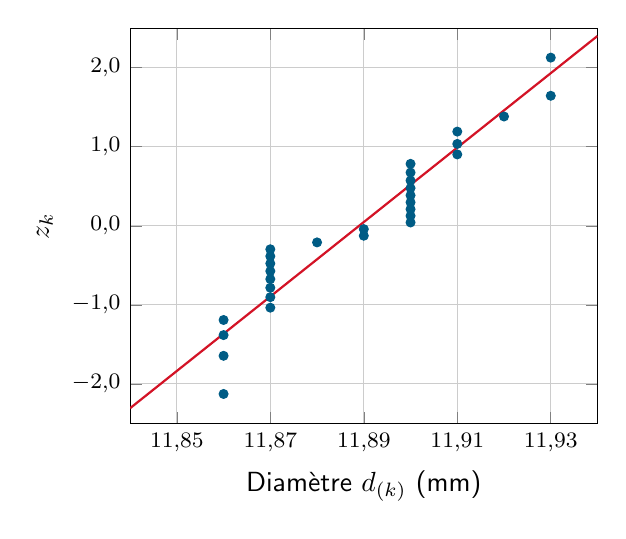
\begin{tikzpicture}
\begin{axis}[width=0.62\linewidth, height=6.6cm, xmin=11.84, xmax=11.94, ymin=-2.5, ymax=2.5, grid=both, grid style={uimmgray!25},
  xlabel={Diamètre $d_{(k)}$ (mm)}, ylabel={$z_k$}, tick label style={font=\footnotesize}, xtick={11.85,11.87,11.89,11.91,11.93},
  /pgf/number format/use comma, /pgf/number format/fixed, /pgf/number format/precision=2, /pgf/number format/fixed zerofill,
  xticklabel style={/pgf/number format/precision=2}, yticklabel style={/pgf/number format/precision=1}, scaled ticks=false]
\addplot[only marks, mark=*, mark size=1.6pt, uimmblue] coordinates {(11.86,-2.128) (11.86,-1.645) (11.86,-1.383) (11.86,-1.192) (11.87,-1.036) (11.87,-0.903) (11.87,-0.784) (11.87,-0.674) (11.87,-0.573) (11.87,-0.477) (11.87,-0.385) (11.87,-0.297) (11.88,-0.210) (11.89,-0.126) (11.89,-0.042) (11.90,0.042) (11.90,0.126) (11.90,0.210) (11.90,0.297) (11.90,0.385) (11.90,0.477) (11.90,0.573) (11.90,0.674) (11.90,0.784) (11.91,0.903) (11.91,1.036) (11.91,1.192) (11.92,1.383) (11.93,1.645) (11.93,2.128)};
\addplot[uimmred, thick, domain=11.84:11.94] {(x-11.889)/0.021229};
\end{axis}
\end{tikzpicture}

{\footnotesize Droite de Henry des $30$ mesures (points) et droite d'une loi normale de même moyenne et de même écart-type $s$ (trait rouge).}
\end{center}
\piege{conclure «~normal~» parce que la plupart des points sont près de la droite~; conclure «~aucune étude n'est possible~» sans chercher l'origine du défaut.}
\end{correction}

% ============================================================
\newpage
\section{Partie B -- Cartes de contrôle}

\needspace{5cm}
\begin{correction}[-- B.1]
\source{\LN{}, §6.1 Énoncé p.~12~; \TDv{}~; \DR{}, §2}
\[
\sigma_{\Dbar} = \frac{\sigma}{\sqrt{5}} = \frac{8{,}6}{2{,}236} \approx 3{,}8 \text{ \textmu m}.
\]
Une moyenne de $5$ pièces varie $\sqrt{5} \approx 2{,}2$ fois moins qu'une pièce~: les écarts, dans un sens et dans l'autre, se compensent en partie. C'est ce qui rend la carte des moyennes sensible aux petits décalages.
\piege{utiliser $\sigma$ à la place de $\sigma/\sqrt{5}$~; diviser par $5$ au lieu de $\sqrt{5}$.}
\end{correction}

\needspace{10cm}
\begin{correction}[-- B.2]
\source{\LN{}, §2.3 p.~5 et §4.1 p.~8 (\texttt{FracNormale})~; \DR{}, §2 et §4}
\begin{enumerate}
  \item $P(Z > z_c) = 0{,}001 \iff P(Z \leq z_c) = 0{,}999$, donc $z_c = \texttt{FracNormale}(0{,}999) \approx 3{,}0902$. De même $P(Z \leq z_s) = 0{,}975$ et $z_s = \texttt{FracNormale}(0{,}975) \approx 1{,}9600$.
  \item $\sigma_{\Dbar} = 0{,}0038453$ mm.
  \[
  LCS = 11{,}889 + 3{,}0902 \times 0{,}0038453 \approx 11{,}901, \qquad LCI = 11{,}889 - 0{,}011883 \approx 11{,}877,
  \]
  \[
  LSS = 11{,}889 + 1{,}9600 \times 0{,}0038453 \approx 11{,}897, \qquad LSI = 11{,}889 - 0{,}007537 \approx 11{,}881.
  \]
  \item $z_c/\sqrt{5} = 3{,}0902/2{,}2361 \approx 1{,}382 = A_c$ et $z_s/\sqrt{5} \approx 0{,}8765$, soit $A_s = 0{,}876$ du tableau à $0{,}001$ près. Les coefficients du tableau ne sont donc pas magiques~: ce sont des seuils de loi normale divisés par $\sqrt{n}$.
  \item $A'_c = A_c/d_n = 1{,}382/2{,}326 = 0{,}594$ et $A'_s = 0{,}377$. Alors
  \[
  \begin{gathered}
  LCS = 11{,}889 + 0{,}594 \times 0{,}020 = 11{,}90088 \approx 11{,}901,\\
  LSI = 11{,}889 - 0{,}377 \times 0{,}020 = 11{,}88146 \approx 11{,}881.
  \end{gathered}
  \]
  Résultats identiques~: c'est normal, car $\Rbar$ remplace $d_n\,\sigma$.
\end{enumerate}
\piege{saisir $0{,}001$ au lieu de $0{,}999$ (résultat $-3{,}09$)~; saisir $0{,}025$ au lieu de $0{,}975$~; oublier de diviser par $\sqrt{n}$ (limites $\pm 3\sigma$ des pièces, trop larges).}
\end{correction}

\needspace{4cm}
\begin{correction}[-- B.3]
\source{\DR{}, §2 et §4}
\[
\begin{gathered}
LC_2 = D'_{c2}\,\Rbar = 2{,}36 \times 0{,}020 = 0{,}0472 \approx 0{,}047 \text{ mm},\\
LS_2 = D'_{s2}\,\Rbar = 1{,}81 \times 0{,}020 = 0{,}0362 \approx 0{,}036 \text{ mm}.
\end{gathered}
\]
\piege{utiliser le tableau des moyennes ($A'_c$, $A'_s$) pour l'étendue.}
\end{correction}

\needspace{9cm}
\begin{correction}[-- B.4]
\source{\DR{}, §2}
\begin{center}
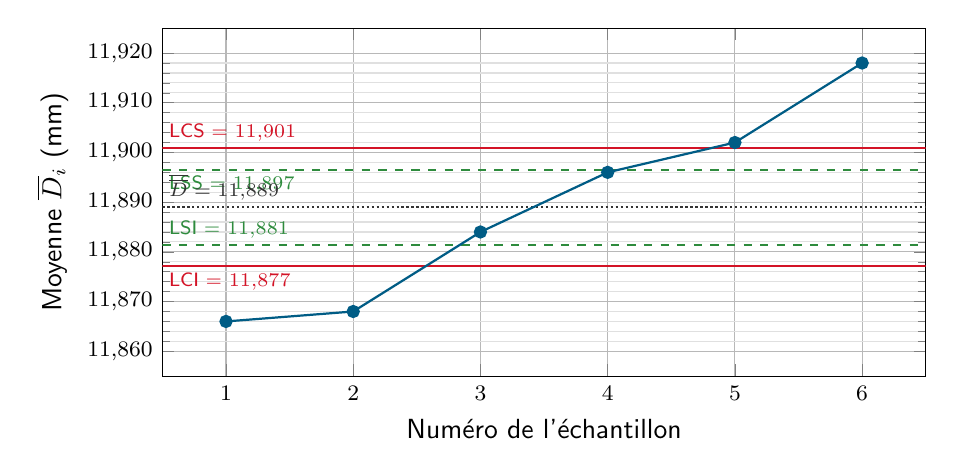
\begin{tikzpicture}
\begin{axis}[ctl, height=6.0cm, ymin=11.855, ymax=11.925, ytick={11.86,11.87,11.88,11.89,11.90,11.91,11.92}, ylabel={Moyenne $\Dbar_i$ (mm)}, yticklabel style={/pgf/number format/precision=3}]
\addplot[uimmred, thick] coordinates {(0.5,11.90088) (6.5,11.90088)} node[pos=0, anchor=south west, font=\scriptsize, text=uimmred, inner sep=2pt] {LCS = $11{,}901$};
\addplot[uimmred, thick] coordinates {(0.5,11.87712) (6.5,11.87712)} node[pos=0, anchor=north west, font=\scriptsize, text=uimmred, inner sep=2pt] {LCI = $11{,}877$};
\addplot[ctlgreen, thick, dashed] coordinates {(0.5,11.89654) (6.5,11.89654)} node[pos=0, anchor=north west, font=\scriptsize, text=ctlgreen, inner sep=2pt] {LSS = $11{,}897$};
\addplot[ctlgreen, thick, dashed] coordinates {(0.5,11.88146) (6.5,11.88146)} node[pos=0, anchor=south west, font=\scriptsize, text=ctlgreen, inner sep=2pt] {LSI = $11{,}881$};
\addplot[uimmgray, thick, densely dotted] coordinates {(0.5,11.889) (6.5,11.889)} node[pos=0, anchor=south west, font=\scriptsize, text=uimmgray, inner sep=2pt] {$\Dbb = 11{,}889$};
\addplot[uimmblue, thick, mark=*, mark size=2pt] coordinates {(1,11.866) (2,11.868) (3,11.884) (4,11.896) (5,11.902) (6,11.918)};
\end{axis}
\end{tikzpicture}
\end{center}
\begin{center}
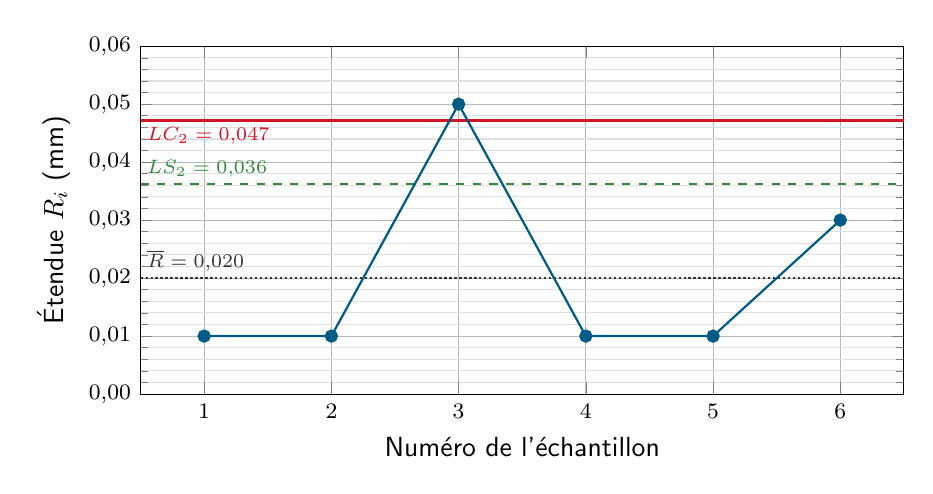
\begin{tikzpicture}
\begin{axis}[ctl, height=6.0cm, ymin=0, ymax=0.06, ytick={0,0.01,0.02,0.03,0.04,0.05,0.06}, ylabel={Étendue $R_i$ (mm)}, yticklabel style={/pgf/number format/precision=2}]
\addplot[uimmred, thick] coordinates {(0.5,0.0472) (6.5,0.0472)} node[pos=0, anchor=north west, font=\scriptsize, text=uimmred, inner sep=2pt] {$LC_2 = 0{,}047$};
\addplot[ctlgreen, thick, dashed] coordinates {(0.5,0.0362) (6.5,0.0362)} node[pos=0, anchor=south west, font=\scriptsize, text=ctlgreen, inner sep=2pt] {$LS_2 = 0{,}036$};
\addplot[uimmgray, thick, densely dotted] coordinates {(0.5,0.020) (6.5,0.020)} node[pos=0, anchor=south west, font=\scriptsize, text=uimmgray, inner sep=2pt] {$\Rbar = 0{,}020$};
\addplot[uimmblue, thick, mark=*, mark size=2pt] coordinates {(1,0.01) (2,0.01) (3,0.05) (4,0.01) (5,0.01) (6,0.03)};
\end{axis}
\end{tikzpicture}
\end{center}
\piege{oublier la ligne centrale~; tracer les limites de la carte des moyennes sur la carte des étendues.}
\end{correction}

\needspace{7cm}
\begin{correction}[-- B.5]
\source{\DR{}, §2}
\textbf{Carte des moyennes.} Les échantillons $1$ ($11{,}866$) et $2$ ($11{,}868$) sont sous $LCI = 11{,}877$. Les échantillons $5$ ($11{,}902$) et $6$ ($11{,}918$) sont au-dessus de $LCS = 11{,}901$. Les échantillons $3$ ($11{,}884$) et $4$ ($11{,}896$) sont dans les limites de surveillance~; le $4$ est juste sous $LSS$. Les moyennes augmentent à chaque échantillon~: six points en hausse continue, d'environ $10$ \textmu m par échantillon.

\textbf{Carte des étendues.} L'échantillon $3$ ($R_3 = 0{,}05$) dépasse $LC_2 = 0{,}047$ et $LS_2 = 0{,}036$. Les autres étendues restent sous $LS_2$.

\textbf{Conclusion.} Le procédé n'est pas maîtrisé~: la moyenne dérive vers le haut, et la dispersion de l'échantillon $3$ est anormale (mesures de $11{,}86$ à $11{,}91$). La carte ne dit pas la cause~: usure d'outil, échauffement, correction du régleur sont des hypothèses à vérifier sur la machine. On ne peut pas se prononcer sur la capabilité tant que le procédé n'est pas stabilisé (voir D.1).
\piege{conclure «~tout est dans la tolérance donc tout va bien~» (aucune mesure n'est hors tolérance, mais ce n'est pas la question)~; ne regarder que la carte des moyennes.}
\end{correction}

\needspace{9cm}
\begin{correction}[-- B.6]
\source{\LD{}, §3.1 Définition p.~7 et §3.4 p.~8 ($P(X \geq 1) = 1 - P(X = 0)$)~; \LN{}, §3.2 p.~6}
\begin{enumerate}
  \item Par construction, $0{,}001$ en haut et $0{,}001$ en bas, soit $0{,}002$ au total.
  \item Les $6$ échantillons sont indépendants, chacun sort des limites avec la probabilité $0{,}002$~: $X \sim \mathcal{B}(6\,;0{,}002)$.
  \[
  P(X \geq 1) = 1 - P(X = 0) = 1 - 0{,}998^{6} \approx 0{,}0119.
  \]
  \item Avoir \emph{au moins un} point hors limites arrive $1{,}2\,\%$ du temps seulement~; en avoir $4$ est quasi impossible ($P(X \geq 4) \approx 2{,}4 \times 10^{-10}$). L'écart-type des $6$ moyennes vaut $20{,}3$ \textmu m, soit $5{,}3$ fois $\sigma_{\Dbar} = 3{,}8$ \textmu m. Les moyennes varient bien plus qu'un procédé stable ne le permet~: il y a une cause identifiable, ce n'est pas le hasard.
\end{enumerate}
\piege{répondre $0{,}002 \times 6 = 0{,}012$ (valeur voisine, mais sans la loi binomiale)~; calculer $P(X = 1)$ au lieu de $P(X \geq 1)$.}
\end{correction}

\needspace{8cm}
\begin{correction}[-- B.7 \textit{(pour aller plus loin)}]
\source{\LN{}, §3.2 p.~6~; \LD{}, §3.4 p.~8}
\begin{enumerate}
  \item Après le décalage, $\Dbar \sim \mathcal{N}(11{,}889 + 0{,}0086\,;0{,}0038453) = \mathcal{N}(11{,}8976\,;0{,}0038453)$.
  \[
  P(\Dbar > LCS) = \texttt{normalFRép}(11{,}90088,\ 10^{99},\ 11{,}8976,\ 0{,}0038453) \approx 0{,}1965.
  \]
  \item Soit $Y$ le nombre d'alarmes sur $5$ échantillons~: $Y \sim \mathcal{B}(5\,;0{,}1965)$ et $P(Y \geq 1) = 1 - (1 - 0{,}1965)^{5} \approx 0{,}665$.
\end{enumerate}
Une dérive de $1\sigma$ (soit $8{,}6$ \textmu m) n'est détectée par la limite de contrôle qu'une fois sur cinq à l'échantillon suivant, et seulement deux fois sur trois sur $5$ échantillons. La limite de surveillance réagit plus tôt~: $P(\Dbar > LSS) \approx 0{,}61$. Pour un décalage de $2\sigma$, la probabilité de dépasser $LCS$ monte à $0{,}92$. C'est la raison d'être des limites de surveillance.
\piege{garder la loi centrée sur $\mu$ après le décalage.}
\end{correction}

% ============================================================
\newpage
\section{Partie C -- Capabilité du procédé}

\needspace{5cm}
\begin{correction}[-- C.1]
\source{\LN{}, §3.2 Calcul d'une probabilité p.~6}
$D \sim \mathcal{N}(11{,}889\,;0{,}0086)$.
\[
P(D < 11{,}85) = \texttt{normalFRép}(-10^{99},\ 11{,}85,\ 11{,}889,\ 0{,}0086) \approx 2{,}9 \times 10^{-6} = 2{,}9 \text{ ppm},
\]
\[
P(D > 12{,}00) = \texttt{normalFRép}(12{,}00,\ 10^{99},\ 11{,}889,\ 0{,}0086) < 10^{-15}, \text{ soit pratiquement } 0 \text{ ppm}.
\]
\piege{oublier $10^{99}$ comme borne et obtenir $0$~; exprimer $2{,}9 \times 10^{-6}$ en pourcentage sans conversion.}
\end{correction}

\needspace{7cm}
\begin{correction}[-- C.2]
\source{\DR{}, §3}
\begin{enumerate}
  \item $IT = 12{,}00 - 11{,}85 = 0{,}15$ mm.
  \[
  C_p = \frac{0{,}15}{6 \times 0{,}0085985} \approx 2{,}91, \qquad
  \frac{T_s - \mu}{3\sigma} = \frac{0{,}111}{0{,}025796} \approx 4{,}30, \qquad \frac{\mu - T_i}{3\sigma} = \frac{0{,}039}{0{,}025796} \approx 1{,}51.
  \]
  $C_{pk} = \min(4{,}30\,;1{,}51) = 1{,}51$.
  \item $1{,}33 \leq 1{,}51 < 2$ : indice \textbf{bon}.
  \item $C_p$ ne regarde que la dispersion, $C_{pk}$ ajoute le centrage. Le milieu de la tolérance est $11{,}925$ et $\mu = 11{,}889$~: le procédé est décentré de $36$ \textmu m vers la borne basse. Centré, il aurait $C_{pk} = C_p = 2{,}91$ (excellent).
\end{enumerate}
\piege{prendre le maximum au lieu du minimum~; calculer $C_p$ avec $\sigma$ au lieu de $6\sigma$~; conclure «~capable~» sans regarder le centrage.}
\end{correction}

\needspace{8cm}
\begin{correction}[-- C.3]
\source{\LN{}, §2.3 p.~5 et §3.2 p.~6~; \DR{}, §3}
\begin{center}
\renewcommand{\arraystretch}{1.3}
\begin{tabular}{|l|c|c|c|c|}\hline
$C_{pk}$ & $1$ & $1{,}33$ & $1{,}67$ & $2$ \\ \hline
$z = 3\,C_{pk}$ & $3$ & $3{,}99$ & $5{,}01$ & $6$ \\ \hline
$P(Z > z)$ en ppm & $1\,350$ & $33{,}0$ & $0{,}27$ & $0{,}001$ \\ \hline
\end{tabular}
\end{center}
$C_{pk} = 1{,}33$ correspond à $z \approx 4$, soit environ $33$ ppm du côté critique~: c'est le seuil de «~procédé capable~» du dossier.

\smallskip
\textbf{Inverse.} $P(Z > z) \leq 10^{-4} \iff P(Z \leq z) \geq 0{,}9999$, donc $z \geq \texttt{FracNormale}(0{,}9999) \approx 3{,}719$ et $C_{pk} \geq 3{,}719/3 = 1{,}2397$. On arrondit par excès~: $C_{pk} \geq 1{,}24$. Avec $1{,}23$, $z = 3{,}69$ et $P \approx 1{,}12 \times 10^{-4}$~: l'exigence n'est pas respectée.
\piege{arrondir à $1{,}23$ (arrondi «~au plus proche~» d'une valeur mal lue)~; saisir $10^{-4}$ comme aire à gauche.}
\end{correction}

\needspace{8cm}
\begin{correction}[-- C.4]
\source{\LN{}, §4.2 Retrouver un paramètre $\mu$ ou $\sigma$ p.~8~; §2.3 p.~5}
Exigence $P(D < T_i) \leq 10^{-4}$~: $\dfrac{T_i - \mu}{\sigma} \leq -3{,}719$, soit $\mu \geq T_i + 3{,}719\,\sigma$.
\begin{enumerate}
  \item $\mu \geq 11{,}85 + 3{,}719 \times 0{,}0085985 = 11{,}88198$. Par excès au micromètre~: $\mu_{\min} = 11{,}882$.
  \item $P(D > T_s) \leq 10^{-4}$ donne $\mu \leq 12{,}00 - 0{,}031983 = 11{,}96802$. Par défaut~: $\mu_{\max} = 11{,}968$.
  \item La fenêtre est $[11{,}882\,;11{,}968]$, de largeur $86$ \textmu m~: c'est $IT$ moins $2 \times 3{,}719\,\sigma \approx 64$ \textmu m. Le réglage actuel $11{,}889$ est dedans, mais à $7$ \textmu m seulement de la borne basse~: marge faible, alors que $C_{pk} = 1{,}51$ paraît confortable.
\end{enumerate}
\piege{arrondir $\mu_{\min}$ à $11{,}881$ ou $\mu_{\max}$ à $11{,}969$ (sens contraire à l'exigence)~; ne traiter qu'un côté.}
\end{correction}

\needspace{6cm}
\begin{correction}[-- C.5]
\source{\LN{}, §4.2 p.~8}
$50$ ppm au total, procédé centré~: $25$ ppm de chaque côté. Il faut $P(D > 12{,}00) \leq 25 \times 10^{-6}$ avec $\mu = 11{,}925$~:
\[
\frac{12{,}00 - 11{,}925}{\sigma} \geq \texttt{FracNormale}(1 - 25 \times 10^{-6}) \approx 4{,}0556 \iff \sigma \leq \frac{0{,}075}{4{,}0556} = 18{,}49 \text{ \textmu m}.
\]
Par défaut au dixième de \textmu m~: $\sigma_{\max} = 18{,}4$ \textmu m. Vérification~: avec $18{,}4$, on obtient $45{,}8$ ppm~; avec $18{,}5$, $50{,}3$ ppm (exigence dépassée). Le procédé actuel ($8{,}6$ \textmu m) a une marge d'un facteur $2{,}1$ \emph{s'il était centré}.
\piege{prendre $50$ ppm de chaque côté~; arrondir à $18{,}5$.}
\end{correction}

% ============================================================
\needspace{9cm}
\section{Partie D -- Synthèse et décision}

\needspace{7cm}
\begin{correction}[-- D.1]
\source{\DR{}, §1 et §3~; \LN{}, §3.1 p.~6}
\begin{enumerate}
  \item $s = 21{,}2$ \textmu m sur les $30$ mesures, soit environ $2{,}5$ fois $\sigma = 8{,}6$ \textmu m.
  \item $C_p' = \dfrac{0{,}15}{6 \times 0{,}021229} \approx 1{,}18$ et $C_{pk}' = \min\!\left(\dfrac{0{,}111}{3 \times 0{,}021229}\,;\dfrac{0{,}039}{3 \times 0{,}021229}\right) = \min(1{,}74\,;0{,}61) \approx 0{,}61$. Avec $C_{pk}' < 1$, le procédé \textbf{n'est pas capable} de tenir toute la production dans la tolérance sur la durée. (On note souvent ces indices «~long terme~» $P_p$ et $P_{pk}$.)
  \item $\sigma = \Rbar/d_n$ mesure la dispersion \emph{à l'intérieur} des échantillons (court terme). $s$ mélange cette dispersion et le déplacement des moyennes d'un échantillon à l'autre, visible sur les cartes (six points en hausse) et sur la droite de Henry (deux paliers). L'écart entre $s$ et $\sigma$ est donc la signature de la dérive.
\end{enumerate}
\piege{retenir seulement $C_{pk} = 1{,}51$ de la partie C~; ne pas relier l'écart à la dérive.}
\end{correction}

\needspace{6cm}
\begin{correction}[-- D.2]
\source{\LN{}, §3.2 p.~6 et §3.3 p.~7}
Avec $\sigma = 0{,}0085985$ mm~:
\[
\begin{gathered}
\text{éch. 1 } (\mu = 11{,}866)\,:\ P(D < 11{,}85) = \texttt{normalFRép}(-10^{99},\,11{,}85,\,11{,}866,\,0{,}0085985) \approx 0{,}0314,\\
\text{éch. 6 } (\mu = 11{,}918)\,:\ P(D < 11{,}85) \approx 1{,}3 \times 10^{-15}.
\end{gathered}
\]
Au départ, le modèle prévoit $3{,}1\,\%$ de pièces sous $T_i$ ($31\,000$ ppm), contre $2{,}9$ ppm pour la moyenne générale. Le $C_{pk}$ global ($1{,}51$) est une moyenne qui masque la situation de départ. Aucune pièce du fichier n'est sous $11{,}85$, ce qui reste cohérent~: sur $5$ pièces, la probabilité de n'en trouver aucune sous $T_i$ est $(1 - 0{,}0314)^5 \approx 0{,}85$.
\piege{conclure que le modèle est faux parce qu'aucune pièce n'est hors tolérance (l'échantillon est trop petit pour le voir).}
\end{correction}

\needspace{7cm}
\begin{correction}[-- D.3]
\source{\LN{}, §4.2 p.~8 (réglage $\mu_{\max}$ de C.4)}
Pente~: $\dfrac{11{,}918 - 11{,}866}{5} = 0{,}0104$ mm, soit $10{,}4$ \textmu m par échantillon. Marge restante jusqu'à $\mu_{\max} = 11{,}968$~: $11{,}968 - 11{,}918 = 0{,}050$ mm. Durée~: $50/10{,}4 \approx 4{,}8$, soit environ $5$ échantillons. C'est un ordre de grandeur tiré de $6$ points, pas une prévision.

\textbf{Actions possibles.} Régleur~: recentrer vers le milieu de la tolérance ($11{,}925$) avec le correcteur d'outil, puis le corriger dès qu'un point sort des limites de surveillance. Technicien méthodes~: rechercher la cause de la dérive (usure de l'outil, échauffement de la broche ou de la pièce, correction manuelle répétée) et resserrer l'intervalle de prélèvement. Après stabilisation, refaire l'étude avec $100$ à $200$ mesures pour calculer $C_p$ et $C_{pk}$ fiables.
\piege{proposer une cause comme un fait établi~; proposer d'élargir la tolérance.}
\end{correction}

\end{document}
